\documentclass[11pt]{article}
\usepackage[a4paper,margin=2.5cm]{geometry}
\usepackage[T1]{fontenc}
\usepackage{lmodern}
\usepackage{amsmath,amssymb,amsthm,bm}
\usepackage{booktabs}
\usepackage{graphicx}
\usepackage{algorithm}
\usepackage{algpseudocode}
\usepackage{natbib}
\usepackage{xcolor}
\usepackage[colorlinks=true,linkcolor=blue!50!black,citecolor=blue!50!black,urlcolor=blue!50!black]{hyperref}
\usepackage{setspace}
\usepackage{caption}
\captionsetup{font=small}
\onehalfspacing

\newtheorem{theorem}{Theorem}
\newtheorem{corollary}{Corollary}
\newtheorem{assumption}{Assumption}
\newtheorem{proposition}{Proposition}

\title{Grouped Decision-Focused Model Averaging for System-Wide Capacity Commitment: Evidence from the U.S.\ Power Grid}
\author{Quang-Vinh Dang\\[2pt]
\small British University Vietnam, Hung Yen, Vietnam\\
\small \href{mailto:vinh.dq4@buv.edu.vn}{vinh.dq4@buv.edu.vn} \quad ORCID: 0000-0002-3877-8024}
\date{}

\begin{document}
\maketitle

\begin{abstract}
\noindent
System planners who coordinate many operating units must commit resources before demand is known, and they typically have several forecasting systems for each unit.
We propose \emph{grouped decision-focused model averaging} (GDMA), which combines the candidate forecasts of many units into commitment rules by jointly learning (i) a small number of latent segments of units and (ii) segment-specific combination weights, chosen to minimise the realised decision cost with unit-specific cost asymmetries rather than forecast error.
A soft version shrinks each unit's own weights towards those of its segment and nests pooled weights, unit-specific weights and shrinkage as special cases.
We derive a finite-sample oracle inequality that separates the cost of learning segment memberships from the cost of learning weights, show that GDMA is asymptotically optimal and attains the risk of the infeasible benchmark with unit-specific optimal weights when segments exist, and prove that it recovers the segments with probability approaching one.
Monte Carlo experiments confirm these properties.
We apply the method to day-ahead capacity commitment for 46 U.S.\ balancing authorities, which together serve 97\% of lower-48 electricity demand, using public hourly data from 2019 to September 2026.
Over six and a half years of out-of-sample operation, soft GDMA lowers system-wide commitment cost by 18--20\% relative to committing on the operators' official forecasts, and by 3--16\% relative to combining the same forecasts for accuracy first; it is the cheapest or statistically tied with the cheapest method for every estimation window.
The learned segments separate operators whose own forecasts carry information beyond recent demand from those for whom machine-learned corrections suffice, a distinction invisible in the organisational structure of the grid.
\par\medskip\noindent\textbf{Keywords:} model averaging; forecast combination; decision-focused learning; latent groups; newsvendor; electricity grid; capacity commitment
\end{abstract}


\section{Introduction}\label{sec:intro}

Electricity systems are managed through many local decision units that commit resources before uncertainty resolves.
Every day, each of the balancing authorities, national system operators and regional market operators that run the world's grids must commit enough capacity to meet the next day's hourly demand.
Committing too little forces expensive real-time purchases, the activation of reserves or, in the worst case, load shedding; committing too much means paying for capacity that sits idle.
The cost of a shortfall is not the same everywhere: an operator embedded in a dense web of interconnections can import from its neighbours, while an isolated system cannot.
Winter Storm Uri in February 2021 is the extreme example: failures of frozen generators and gas supply forced the weakly interconnected Texas grid to shed load for days, and its limited ability to import deepened the crisis, while neighbouring systems with more import capability shed much less \citep{Busby2021,FERCNERC2021}.
At the same time, governments are committing to large battery-storage programmes, and planners must decide where those batteries should go.

Operators and planners do not lack forecasts.
Operators publish their own day-ahead forecasts, simple persistence and calendar rules are always available, statistical and machine-learning models can be trained on the data, and pretrained foundation models now forecast any series zero-shot \citep{Ansari2024chronos}.
None dominates everywhere, which makes combining them attractive.
How to combine them is less obvious.
The forecast-combination and model-averaging literature, from \citet{BatesGranger1969} to the asymptotic theory of \citet{Hansen2007}, \citet{HansenRacine2012}, \citet{ZhangWanZou2013} and \citet{ZhangLiu2023}, offers two options when there are many series.
Weights can be estimated series by series, which respects heterogeneity but produces noisy weights when histories are short---the root of the ``forecast-combination puzzle'' that simple averages often beat estimated weights \citep{SmithWallis2009,Claeskens2016}.
Or one set of weights can be estimated for all series, which is precise but imposes the same rule on systems that face different conditions.
Deep learning offers a third option, a network that maps features to weights \citep{MonteroManso2020,Gong2026moe}, at the price of thousands of parameters and weights that are hard to audit.
All three typically judge a combination by its statistical accuracy, although the planner is judged by the cost of the resulting decisions; the decision-focused literature in operations management has shown that learning directly for the decision can be much better than forecasting accurately and then optimising \citep{BanRudin2019,BertsimasKallus2020,ElmachtoubGrigas2022}.

This paper proposes \emph{grouped decision-focused model averaging} (GDMA) and uses it to answer three management questions: how should grid operators on five continents combine the forecasts they have into day-ahead capacity commitments, who gains and who loses from a common planning rule, and where should new batteries be installed?
GDMA assumes that decision units fall into a small number of latent segments whose members are best served by the same combination of candidate rules, and estimates the segments and the segment-specific weights jointly by minimising the realised system-wide decision cost, in money, with each unit's own cost asymmetry.
A soft version shrinks each unit's own weights towards those of its segment.
The number of segments and the shrinkage intensity are chosen by a time-ordered hold-out.
Pooled weights, unit-specific weights and shrinkage towards pooled weights are special cases, and the combined commitment is always a convex combination of commitments the operator already understands.
A second, planning stage takes the residual shortfall risk left by the learned rule and allocates a storage budget across grid areas.

\begin{figure}[t]
\centering
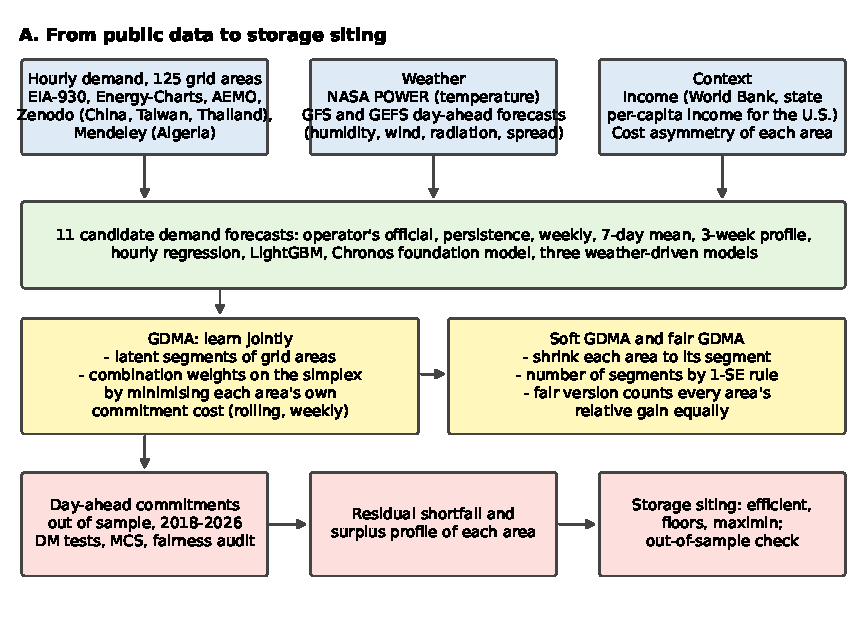
\includegraphics[width=0.9\textwidth]{figures/fig_pipeline.pdf}
\caption{The approach from public data to storage siting.}\label{fig:pipeline}
\end{figure}

\begin{figure}[t]
\centering
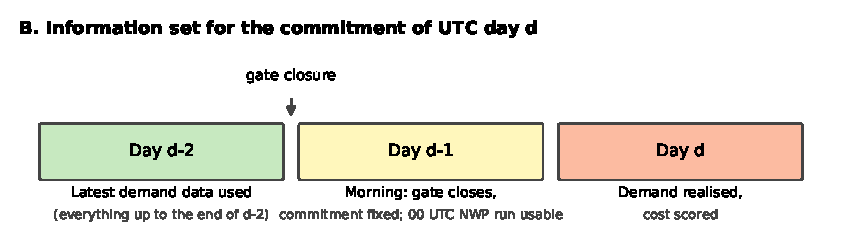
\includegraphics[width=0.95\textwidth]{figures/fig_timeline.pdf}
\caption{Information set of the day-ahead commitment. Data up to the end of day $d-2$ and the 00~UTC weather forecast of day $d-1$ (only where it is available before gate closure) enter the commitment for day $d$.}\label{fig:timeline}
\end{figure}

Figure~\ref{fig:pipeline} summarises the approach and Figure~\ref{fig:timeline} the timing of the information.

We make five contributions.
\begin{enumerate}
\item \textbf{Method.} We formulate the joint learning of latent segments and combination weights under an asymmetric, unit-specific decision loss, give a $k$-means-type algorithm with regret-space seeding in which every step is a small convex program, and link it to a storage-siting problem that is solved exactly by a greedy algorithm (Section~\ref{sec:method}).
To our knowledge, neither the model-averaging, the decision-focused learning nor the latent-group panel literature \citep{BonhommeManresa2015,Su2016} has proposed this estimator.
\item \textbf{Learning theory.} We prove a finite-sample oracle inequality that separates the cost of learning memberships ($\log G/T$ per unit) from the cost of learning weights ($GM\log(NT)/(NT)$), which shows how the cost of grouping scales relative to unit-specific weights when histories are short; we show that GDMA is asymptotically optimal and, under a segment structure, attains the risk of the infeasible benchmark in which every unit knows its own optimal weights; that it recovers the segments with probability approaching one; and that on this event it coincides exactly with an estimator told the segments (Section~\ref{sec:theory}).
\item \textbf{Evidence on five continents.} We evaluate all rules with the information available at the day-ahead gate closure. On 46 U.S.\ balancing authorities with their official forecasts (Section~\ref{sec:app}) and on a global panel of 125 grid areas in North America, Europe, Oceania, Asia and Africa (Section~\ref{sec:global}), soft GDMA lowers the stylised out-of-sample commitment cost by 13--17\% relative to the official forecasts in the United States and by 12\% worldwide relative to a reference forecaster, beats combining the same forecasts for accuracy by 2--3 points in the United States (at $W=28$) and 8--10 points worldwide, and beats a decision-focused neural mixture-of-experts gate by seven percentage points worldwide. Decision-focused shrinkage and two-step clustering come close, and a model confidence set cannot separate the grouped variants from one another, so the evidence is for decision-focused combination with cross-sectional structure rather than for grouping alone. A pretrained foundation model and models driven by archived day-ahead deterministic and ensemble weather forecasts enter the candidate set on equal terms; the ensemble information roughly halves, but does not close, the gap to the operators' own forecasts during Winter Storm Elliott, the most abrupt event in the sample.
\item \textbf{Fairness.} We audit how the gains are distributed across grid areas and propose a fair variant that counts every area's relative improvement equally. Soft GDMA makes 6\% of areas worse off than their own best candidate, against 24\% for pooled weights and 42\% for the neural gate, shows no systematic gradient with national or state income that the data can detect, and its fair variant halves the share of areas made worse off at no cost in total (Section~\ref{sec:fairaudit}).
\item \textbf{Storage siting.} In a stylised storage model, better commitment rules reduce what storage can add: the reference rule needs 34\,GW of optimally sited batteries to reach the cost that soft GDMA achieves without any. The optimal location of a storage programme depends on the commitment rule, but siting on the wrong rule's error profile loses only 2--4\% of a programme's value, and maximin-fair siting helps the worst-served continent at a price of fairness of 7--9\% (Section~\ref{sec:storage}).
\end{enumerate}

The paper speaks to the theme of this special issue in both directions it describes: it develops a statistical learning method with guarantees, motivated by a concrete management problem, and it uses new, openly available data and models to answer a planning question of continental scale.
Replication code and data-construction scripts are available in a public repository (see the data availability statement).

\section{Related literature and the research gap}\label{sec:lit}

\paragraph{Model averaging and forecast combination}
Since \citet{BatesGranger1969}, combining forecasts has been one of the most reliable ways to improve accuracy; \citet{Timmermann2006} and \citet{Wang2023review} review five decades.
Frequentist model averaging chooses weights by minimising estimated risk---a Mallows criterion \citep{Hansen2007}, leave-one-out or $K$-fold cross-validation \citep{HansenRacine2012,ZhangLiu2023}, or forward validation for time series \citep{ZhangZhang2023}---and establishes asymptotic optimality: the chosen weights attain the lowest attainable risk.
It now covers dependent data \citep{ZhangWanZou2013}, quantile losses \citep{LuSu2015}, general losses \citep{Yu2024unified}, time-varying weights \citep{Sun2021tvma}, covariate-dependent weights \citep{Gong2026moe}, covariate shift \citep{Zhang2026shift} and prediction intervals \citep{Qu2025intervals}.
The forecast-combination puzzle, that equal weights frequently beat estimated weights, is attributed mainly to estimation error \citep{SmithWallis2009,Claeskens2016}; remedies shrink weights towards equal weights \citep{DieboldShin2019} or restrict them \citep{Zou2025weights}.
With many series, weights are estimated series by series or learned from series features \citep[FFORMA,][]{MonteroManso2020}; \citet{AiolfiTimmermann2006} cluster \emph{forecasting models} by past performance.
All of these treat each target series separately or impose one rule on all, and none groups the \emph{target units}.

\paragraph{Decision-focused learning}
The loss that matters is the decision cost \citep{Granger1969}.
The data-driven newsvendor literature learns order quantities directly from data \citep{Levi2015,BanRudin2019}, prescriptive analytics maps covariates to decisions \citep{BertsimasKallus2020}, and ``smart predict-then-optimise'' trains predictors on decision regret \citep{ElmachtoubGrigas2022}; see \citet{Mandi2024} for a survey.
In energy forecasting, \citet{Wang2019cqra} combine probabilistic load forecasts by minimising pinball loss on the simplex, one series at a time.
Most of this work concerns single models or one unit; the exception is data pooling \citep{GuptaKallus2022}, which shrinks the solutions of many small newsvendor-type problems towards a common anchor, which pays even for unrelated problems; decision-focused shrinkage of weights towards pooled weights, one of our benchmarks and the $G=1$ case of soft GDMA, applies the same idea to forecast combination.

\paragraph{Deep learning for forecasting and for combination weights}
Pretrained foundation models such as Chronos \citep{Ansari2024chronos} forecast unseen series zero-shot with accuracy close to trained models, and deep networks increasingly \emph{produce} combination weights: FFORMA maps series features to weights with gradient boosting \citep{MonteroManso2020}, and mixture-of-experts model averaging uses a softmax neural gate \citep{Gong2026moe}.
These approaches are flexible, but fit thousands of parameters, give weights that are hard to audit and, except for \citet{Gong2026moe}, lack optimality guarantees for the combined decision.
We include a foundation model as a candidate and a decision-focused neural gate as a competitor.

\paragraph{Storage siting}
Battery siting is usually decided with engineering models of the transmission network, solved by decomposition or stochastic programming \citep{Piansky2024battery,Larroux2026bess}, which take the uncertainty storage must absorb as an input.
We make that input endogenous: residual commitment risk depends on how operators combine forecasts, so the value and best location of storage depend on the forecasting policy.

\paragraph{Latent group structures}
Panel econometrics models unobserved heterogeneity through latent groups estimated by $k$-means-type algorithms \citep{LinNg2012,BonhommeManresa2015,AndoBai2016} or classifier-Lasso \citep{Su2016}.
\citet{GuVolgushev2019} extend latent groups to panel quantile regression, the closest statistical relative of GDMA: a grouped quantile regression of demand on the candidate forecasts would be an unconstrained version of our quantile-regression benchmark.
These methods group regression parameters, typically fixed effects, for inference on the parameters; GDMA groups simplex weights over existing forecasting systems, with unit-specific critical ratios, and is judged by the out-of-sample cost of its decisions.

\paragraph{The gap}
Table~\ref{tab:gap} summarises the position of GDMA.
No existing method simultaneously (a) combines a library of existing candidate rules, including machine-learning and foundation-model forecasts, (b) chooses weights by the downstream decision cost with unit-specific cost asymmetries, and (c) shares strength across many decision units through latent segments whose number is chosen from data, with guarantees on optimality and segment recovery; nor does any link the resulting operational risk to the siting of new storage.
The ingredients exist---decision-focused combination, shrinkage across problems, latent groups---and the contribution is their combination, the theory for it, and its use for a planning decision; much of the gain over the best single forecaster is already delivered by decision-focused shrinkage, and grouping adds a smaller refinement.
The gap matters most when windows are short, because systems change and old data are stale, and units are many, as in infrastructure planning.

\begin{table}[t]
\centering
\caption{Positioning of GDMA relative to existing approaches.}\label{tab:gap}
\footnotesize
\begin{tabular}{@{}p{6.2cm}cccc@{}}
\toprule
 & Combines & Decision- & Shares strength & Heterogeneous \\
Approach & candidates & focused loss & across units & weights \\
\midrule
Per-series combination / JMA / forward validation & \checkmark & & & \checkmark \\
Pooled combination & \checkmark & & \checkmark & \\
Quantile / general-loss model averaging & \checkmark & \checkmark & & \checkmark \\
Shrinkage towards equal or pooled weights & \checkmark & & partial & \checkmark \\
Data pooling in stochastic optimisation & & \checkmark & partial & \checkmark \\
Feature-based weights (FFORMA) & \checkmark & & \checkmark & \checkmark \\
Neural mixture-of-experts gate & \checkmark & (\checkmark) & \checkmark & \checkmark \\
Data-driven newsvendor, SPO & & \checkmark & \checkmark & \\
Latent-group panel (quantile) models & & (\checkmark) & \checkmark & \checkmark \\
\textbf{GDMA (this paper)} & \checkmark & \checkmark & \checkmark & \checkmark \\
\bottomrule
\end{tabular}
\end{table}

\section{Grouped decision-focused model averaging}\label{sec:method}

\subsection{The system-wide commitment problem}

A planner is responsible for $N$ decision units (in our application the balancing authorities of the U.S.\ grid).
In period $t$ unit $i$ must commit a quantity $q_{it}$ before demand $y_{it}$ is realised.
Committing too little costs $u_i>0$ per unit of shortfall (emergency purchases, reserve activation or, in the limit, curtailed load); committing too much costs $o_i>0$ per unit of excess (idle capacity that was paid for).
The period cost is the newsvendor cost
\begin{equation}\label{eq:cost}
C_i(q,y)=u_i\,(y-q)^+ + o_i\,(q-y)^+ = (u_i+o_i)\,\rho_{\tau_i}(y-q),\qquad \tau_i=\frac{u_i}{u_i+o_i},
\end{equation}
where $\rho_\tau(r)=r(\tau-\mathbb 1\{r<0\})$ is the check function.
The system cost that the planner cares about is $\sum_i\sum_t C_i(q_{it},y_{it})$; under~\eqref{eq:cost} the cost-minimising commitment is the conditional $\tau_i$-quantile of demand \citep{Gneiting2011}.
Critical ratios $\tau_i$ differ across units because the consequences of a shortfall differ: an operator that is tightly interconnected with its neighbours can import at moderate cost, while an isolated one cannot.

For every unit a library of $M$ candidate commitment rules is available.
Candidate $m$ proposes $q^{(m)}_{it}$, computed from information available before period $t$; we write $\bm q_{it}=(q^{(1)}_{it},\dots,q^{(M)}_{it})^\top$.
The candidates may come from any source: an operator's own published forecast, simple persistence rules, statistical models or machine-learning models, each turned into a commitment by adding its own $\tau_i$-quantile residual margin.
The planner combines them linearly,
\[
q_{it}(\bm w)=\bm q_{it}^\top\bm w,\qquad \bm w\in\Delta_M=\Big\{\bm w\in\mathbb R^M:\ w_m\ge 0,\ \textstyle\sum_m w_m=1\Big\}.
\]
The simplex constraint keeps the combined commitment inside the range spanned by the candidates, which is what makes the combination interpretable and auditable by operators, and it is known to stabilise estimated weights \citep{Zou2025weights}.

\subsection{Three ways to estimate the weights}

Let the estimation window contain periods $t=1,\dots,T$ for which both candidate commitments and realised demand are observed (a forward-validation sample in the terminology of \citealp{ZhangZhang2023}).
Write $\widehat R_i(\bm w)=T^{-1}\sum_{t=1}^T C_i(\bm q_{it}^\top\bm w,y_{it})$ for the empirical cost of unit $i$.

\paragraph{Unit-specific weights.} $\widehat{\bm w}_i=\arg\min_{\bm w\in\Delta_M}\widehat R_i(\bm w)$.
This respects heterogeneity but estimates $M-1$ free parameters from $T$ serially dependent observations per unit; it is the decision-focused counterpart of per-series forecast combination, and suffers from the same estimation noise that underlies the forecast-combination puzzle \citep{SmithWallis2009,Claeskens2016}.

\paragraph{Pooled weights.} $\widehat{\bm w}=\arg\min_{\bm w}\sum_i\widehat R_i(\bm w)$.
This uses all $NT$ observations but forces a single policy on units that may need different ones.

\paragraph{Grouped weights (proposed).}
We posit that units fall into a small number $G$ of latent segments whose members are well served by the same combination.
The GDMA estimator solves
\begin{equation}\label{eq:gdma}
(\widehat{\bm\gamma},\widehat{\bm W})=\arg\min_{\bm\gamma\in\{1,\dots,G\}^N,\ \bm W=(\bm w_1,\dots,\bm w_G)\in\Delta_M^G}\ \sum_{i=1}^N\sum_{t=1}^T C_i\big(\bm q_{it}^\top\bm w_{\gamma_i},\,y_{it}\big),
\end{equation}
and unit $i$ commits $\bm q_{i,T+1}^\top\widehat{\bm w}_{\widehat\gamma_i}$.
$G=1$ gives pooled weights and $G=N$ gives unit-specific weights, so the number of segments indexes the whole range between the two extremes.
Three features separate~\eqref{eq:gdma} from existing proposals.
First, the criterion is the decision cost in the planner's own units (money or energy), so units are grouped by \emph{how they should act}, not by how their forecasts look.
Second, memberships and weights are estimated jointly; a two-step procedure that clusters noisy unit-specific weights and then re-estimates is a natural but inferior alternative (Section~\ref{sec:sim}).
Third, because each unit keeps its own critical ratio and its own candidate margins, units in one segment share a combination rule but not a commitment level.

\subsection{Computation}

Problem~\eqref{eq:gdma} is a mixed-integer problem, but it has the structure of $k$-means with a non-Euclidean, data-dependent distortion, as in the grouped fixed-effects estimator of \citet{BonhommeManresa2015}.
Given memberships, the weights of each segment solve a pooled convex problem on the simplex; given weights, each unit joins the segment whose weights give it the lowest in-window cost.
Algorithm~\ref{alg:gdma} alternates the two steps.
The weight step is a linear program; for speed we minimise a softplus-smoothed check function,
$\rho^\varepsilon_\tau(r)=\tau r+\varepsilon\log(1+e^{-r/\varepsilon})$, with bandwidth $\varepsilon$ equal to $2\%$ of the unit's typical decision error, by sequential quadratic programming.
On our data the smoothed solution is within $0.01\%$ of the exact linear-programming optimum in cost.
Each iteration weakly decreases the objective, so the algorithm converges to a local solution in finitely many steps; we run several starts and keep the best.
Starting values are drawn by a $k$-means++ rule \citep{ArthurVassilvitskii2007} in \emph{regret space}: the next seed unit is drawn with probability proportional to the extra cost that units would incur if forced to use the closest existing seed's own weights.
In rolling applications the memberships of the previous window provide an additional warm start.

\begin{algorithm}[t]
\caption{GDMA for a fixed number of segments $G$}\label{alg:gdma}
\begin{algorithmic}[1]
\Require candidate commitments $\{\bm q_{it}\}$, demand $\{y_{it}\}$, costs $\{u_i,o_i\}$, $G$, number of starts $S$
\State compute unit-specific weights $\widehat{\bm w}_i$ and the regret matrix $D_{ij}=\widehat R_i(\widehat{\bm w}_j)-\widehat R_i(\widehat{\bm w}_i)$
\For{$s=1,\dots,S$}
  \State draw seeds $j_1,\dots,j_G$ by $k$-means++ on $D$ and set $\bm w_g\gets\widehat{\bm w}_{j_g}$
  \Repeat
    \State $\gamma_i\gets\arg\min_g\widehat R_i(\bm w_g)$ for all $i$ \Comment{assignment step}
    \State re-seed any empty segment with the unit of largest regret
    \State $\bm w_g\gets\arg\min_{\bm w\in\Delta_M}\sum_{i:\gamma_i=g}\widehat R_i(\bm w)$ for all $g$ \Comment{pooled convex step}
  \Until{memberships do not change}
\EndFor
\State \Return the solution with the lowest objective~\eqref{eq:gdma}
\end{algorithmic}
\end{algorithm}

\subsection{Soft segments}\label{sec:soft}

Segments need not be exact.
When units within a segment are similar but not identical, a unit may benefit from a rule that sits between its own estimated weights and those of its segment.
\emph{Soft GDMA} uses
\begin{equation}\label{eq:soft}
\widehat{\bm w}^{\,\mathrm{soft}}_i=(1-\kappa)\,\widehat{\bm w}_i+\kappa\,\widehat{\bm w}_{\widehat\gamma_i},\qquad\kappa\in[0,1],
\end{equation}
where $\widehat{\bm w}_i$ are the unit-specific weights and $\widehat{\bm w}_{\widehat\gamma_i}$ the GDMA weights of the unit's segment.
Because the simplex is convex, $\widehat{\bm w}^{\,\mathrm{soft}}_i\in\Delta_M$.
The family nests every benchmark: $\kappa=1$ is GDMA, $\kappa=0$ is unit-specific weights, $G=1$ is shrinkage towards pooled weights (a decision-focused analogue of \citealp{DieboldShin2019}), and $G=1,\kappa=1$ is pooled weights.
The pair $(G,\kappa)$ is chosen jointly by the hold-out described next, over $G\in\{1,\dots,G_{\max}\}$ and $\kappa\in\{0,0.25,0.5,0.75,1\}$.
Segment centres play the role of data-driven prior means, in the spirit of empirical Bayes shrinkage towards group-specific targets.

\subsection{Choosing the number of segments}

We split the estimation window into an early block (the first two thirds) and a late block.
For each $G\in\{1,\dots,G_{\max}\}$ we estimate~\eqref{eq:gdma} on the early block and record every unit's cost on the late block under its estimated membership and weights.
Let $G^\dagger$ minimise the total late-block cost.
Following the one-standard-error rule \citep{HastieTibshiraniFriedman2009}, we choose the smallest $G$ whose total late-block cost exceeds that of $G^\dagger$ by no more than one standard error of the summed unit-level cost differences, and then re-estimate on the full window.
The rule respects time order and prefers parsimonious segmentations, which are easier to explain to the operators who would have to adopt them.
For soft GDMA we simply take the pair $(G,\kappa)$ with the lowest late-block cost.

\section{Theoretical properties}\label{sec:theory}

This section studies the global minimiser of~\eqref{eq:gdma} for a given $G$.
We show that (i) its expected decision cost is close to that of the best grouped policy, with an estimation error that separates the price of learning memberships from the price of learning weights; (ii) it is asymptotically optimal and, under a latent segment structure, attains the risk of the infeasible unit-specific oracle; and (iii) it recovers the segments with probability approaching one, in which case its weights coincide with those of an estimator that is told the segments.
Proofs are in Appendix~\ref{app:proofs}.

\subsection{Setting and assumptions}

Let $\bm z_{it}=(y_{it},\bm q_{it})$.
Define the population risk of unit $i$, $R_i(\bm w)=\mathbb E\,C_i(\bm q_{it}^\top\bm w,y_{it})$, and for a grouped policy $(\bm\gamma,\bm W)$ the average risk and its empirical analogue
\[
R(\bm\gamma,\bm W)=\frac1N\sum_{i=1}^N R_i(\bm w_{\gamma_i}),\qquad
\widehat R(\bm\gamma,\bm W)=\frac1{NT}\sum_{i=1}^N\sum_{t=1}^T C_i(\bm q_{it}^\top\bm w_{\gamma_i},y_{it}).
\]
Let $\mathcal P_G=\{1,\dots,G\}^N\times\Delta_M^G$ and $R^*_G=\inf_{\mathcal P_G}R$.

\begin{assumption}[Stationarity and boundedness]\label{as:bounded}
For each $i$, $\{\bm z_{it}\}_t$ is strictly stationary, $|y_{it}|\le B$ and $\|\bm q_{it}\|_\infty\le B$ almost surely, and $\max_i(u_i+o_i)\le\bar a$.
\end{assumption}

Stationarity refers to the candidate commitments as well as demand; it holds, for instance, when every candidate is computed from a rolling window of fixed length of a stationary process.
Boundedness is natural once demand is normalised by a unit's scale.
Under Assumption~\ref{as:bounded} each loss lies in $[0,L]$ with $L=2\bar aB$ and is Lipschitz in the weights: $|C_i(\bm q^\top\bm w,y)-C_i(\bm q^\top\bm w',y)|\le\bar aB\|\bm w-\bm w'\|_1$.

\begin{assumption}[Concentration]\label{as:concentration}
There are constants $c>0$ and an effective sample length $T_e\le T$ such that, for every fixed $(\bm\gamma,\bm W)\in\mathcal P_G$ and every $x>0$,
\[
\Pr\big(|\widehat R(\bm\gamma,\bm W)-R(\bm\gamma,\bm W)|>x\big)\le 2\exp\!\big(-c\,N T_e\,x^2/L^2\big),
\]
and, for every $i$ and fixed $\bm w$, $\Pr(|\widehat R_i(\bm w)-R_i(\bm w)|>x)\le 2\exp(-c\,T_e\,x^2/L^2)$.
\end{assumption}

Assumption~\ref{as:concentration} is a high-level condition.
It holds with $T_e=T$ when observations are independent (Hoeffding's inequality) and, when units are independent and each $\{\bm z_{it}\}_t$ is geometrically $\beta$-mixing, with $T_e=T/(C\log T)$ by the blocking argument of \citet{Yu1994} or the Bernstein inequality of \citet{Merlevede2011}.
Cross-sectional dependence through common shocks (weather, in our application) reduces the effective number of independent units; the results continue to hold with $N$ replaced by an effective cross-sectional size.

\subsection{An oracle inequality}

\begin{theorem}[Oracle inequality]\label{thm:oracle}
Let Assumptions~\ref{as:bounded}--\ref{as:concentration} hold and let $(\widehat{\bm\gamma},\widehat{\bm W})$ be a global minimiser of~\eqref{eq:gdma}.
For any $\delta\in(0,1)$, with probability at least $1-\delta$,
\begin{equation}\label{eq:oracle}
R(\widehat{\bm\gamma},\widehat{\bm W})\le R^*_G+2L\sqrt{\frac{GM\log(3NT_e)+N\log G+\log(2/\delta)}{c\,NT_e}}+\frac{4\bar aB}{NT_e}.
\end{equation}
\end{theorem}

The square-root term has a transparent decomposition.
Per unit, learning the segment membership costs $\log G/T_e$, while learning the segment weights costs $GM\log(NT_e)/(NT_e)$.
The same argument applied to unit-specific weights ($G=N$) gives $M\log(NT_e)/T_e$, and applied to pooled weights ($G=1$) gives $M\log(NT_e)/(NT_e)$ but a larger approximation error $R^*_1-R^*_N$.
Grouping therefore replaces the $M$ per-unit parameters of unit-specific weights by a single discrete label that costs $\log G$ rather than $M\log(NT_e)$ to learn.
This is the formal sense in which GDMA resolves the tension between the noise of unit-specific weights and the bias of pooled weights: with $M=7$ candidates, $N=46$ units, $G=4$ segments and an effective length of $T_e=28$ (one observation per day of a four-week window), the variance proxy under the square root is $0.23$ for GDMA against $2.07$ for unit-specific weights, so the bound is about three times tighter, while the approximation error of GDMA is zero whenever the segment structure is correct.

\subsection{Asymptotic optimality}

Following the model-averaging literature \citep{Hansen2007,HansenRacine2012,ZhangLiu2023}, call a weight choice asymptotically optimal if the ratio of its risk to the lowest attainable risk in its class tends to one.

\begin{corollary}[Asymptotic optimality]\label{cor:ao}
Let the assumptions of Theorem~\ref{thm:oracle} hold, with $G$ and $M$ possibly growing, and suppose $R^*_G\ge\kappa>0$.
If $GM\log(NT_e)/(NT_e)\to0$ and $\log G/T_e\to0$, then
$R(\widehat{\bm\gamma},\widehat{\bm W})/R^*_G\to_p1$.
If, in addition, there are memberships $\bm\gamma^0$ with $G_0\le G$ segments such that $\arg\min_{\bm w}R_i(\bm w)$ depends on $i$ only through $\gamma^0_i$, then $R^*_G=R^*_N=N^{-1}\sum_i\min_{\bm w}R_i(\bm w)$ and
\[
\frac{R(\widehat{\bm\gamma},\widehat{\bm W})}{N^{-1}\sum_{i}\min_{\bm w\in\Delta_M}R_i(\bm w)}\to_p1 .
\]
\end{corollary}

The second statement is the relevant one for practice: under a segment structure, GDMA attains the risk of the infeasible benchmark in which every unit knows its own optimal weights, although it estimates only $G(M-1)$ continuous parameters.
Unit-specific weights attain the same limit only if $M\log(NT_e)/T_e\to0$, a much stronger requirement when windows are short because the system is non-stationary and old data are of limited use.
The condition $R^*_G\ge\kappa$ excludes the degenerate case of perfect foresight, which never occurs in commitment problems.

\subsection{Recovery of the segments}

\begin{assumption}[Segment structure]\label{as:groups}
(a) There are $\bm\gamma^0\in\{1,\dots,G\}^N$ and distinct $\bm w^0_1,\dots,\bm w^0_G\in\Delta_M$ such that, for all $i$ and all $\bm w\in\Delta_M$, $R_i(\bm w)-R_i(\bm w^0_{\gamma^0_i})\ge\lambda\|\bm w-\bm w^0_{\gamma^0_i}\|_2^2$ for some $\lambda>0$.
(b) $\min_{g\ne h}\|\bm w^0_g-\bm w^0_h\|_2\ge d>0$ and every segment contains at least $\pi N$ units, $\pi>0$.
\end{assumption}

Part~(a) is a quadratic-growth condition.
It holds when the conditional density of demand given the candidates is bounded away from zero near the optimal commitment and the candidates are not collinear, because the Hessian of $R_i$ is then $(u_i+o_i)\,\mathbb E[f_{y|\bm q}(\bm q^\top\bm w)\,\bm q\bm q^\top]$, which is positive definite on the tangent space of the simplex.
Part~(b) requires segments to be genuinely different and non-negligible, as in \citet{BonhommeManresa2015}.

\begin{theorem}[Segment recovery and oracle equivalence]\label{thm:recovery}
Let Assumptions~\ref{as:bounded}--\ref{as:groups} hold with $G$ equal to the true number of segments, and let $N,T_e\to\infty$ with $\log N/T_e\to0$.
Then, up to a relabelling of segments,
(i) $\max_g\|\widehat{\bm w}_g-\bm w^0_g\|_2\to_p0$;
(ii) $\Pr(\widehat{\bm\gamma}\ne\bm\gamma^0)\le N\,C_M\exp(-c'T_e)+o(1)\to0$ for constants $C_M,c'>0$ that do not depend on $N$ or $T$;
(iii) with probability approaching one, $\widehat{\bm W}$ equals the infeasible estimator $\widetilde{\bm W}=\arg\min_{\bm W}\widehat R(\bm\gamma^0,\bm W)$ that knows the segments.
\end{theorem}

Part~(iii) is an exact equivalence, not an asymptotic approximation: on the event that memberships are recovered, the joint minimiser and the known-segment minimiser are the same object.
Any distributional result available for the known-segment estimator therefore transfers to GDMA without modification.
The recovery condition $\log N/T_e\to0$ is mild: the number of units may grow polynomially in the window length.

\paragraph{Soft GDMA.}
For fixed $(G,\kappa)$, $R_i$ is convex in $\bm w$, so the risk of~\eqref{eq:soft} satisfies
$R_i(\widehat{\bm w}^{\,\mathrm{soft}}_i)\le(1-\kappa)R_i(\widehat{\bm w}_i)+\kappa R_i(\widehat{\bm w}_{\widehat\gamma_i})$.
Averaging over units, the excess risk of soft GDMA is at most the $\kappa$-weighted average of the excess risks of unit-specific weights and of GDMA, each controlled by Theorem~\ref{thm:oracle}.
Under a segment structure, therefore, any $\kappa$ bounded away from zero inherits the faster rate of GDMA for the $\kappa$ share of the combination, while $\kappa<1$ buys robustness when segments are only approximate.
Choosing $(G,\kappa)$ from a finite grid by hold-out adds only a $\log(|\mathcal G|)$ term to the hold-out error, where $|\mathcal G|$ is the grid size.


\paragraph{Weighted and fair criteria.}
All results of this section hold for criteria in which unit $i$'s costs are multiplied by a weight $\omega_i\in[\underline\omega,\bar\omega]$ with $0<\underline\omega\le\bar\omega<\infty$: the weights only rescale $u_i$ and $o_i$, so Assumptions~\ref{as:bounded}--\ref{as:groups} hold with $\bar a$ replaced by $\bar\omega\bar a$ and $\lambda$ by $\underline\omega\lambda$.
Fair soft GDMA uses data-dependent weights $\omega_i\propto1/c_i^0$; treating them as fixed within a window, Theorem~\ref{thm:oracle} bounds its weighted excess risk.
Under the segment structure of Corollary~\ref{cor:ao}, the weighted and unweighted criteria have the same minimiser, because every unit attains its own optimal weights, and since each unit's excess risk is non-negative the unweighted excess risk is at most $1/\underline\omega$ times the weighted one (weights normalised to mean one).
Fairness then costs nothing asymptotically.
When segments are only approximate, the fair criterion trades some total cost for a more even distribution of the gains; this is the price of fairness that we measure empirically.

\section{Monte Carlo evidence}\label{sec:sim}

PENDING

\section{Day-ahead capacity commitment on the U.S.\ grid}\label{sec:app}

\subsection{Data}

We use the complete public record of the U.S.\ Energy Information Administration's Hourly Electric Grid Monitor (Form EIA-930; \citealp{EIA930}), downloaded on 29 September 2026.
For every balancing authority (BA) in the lower 48 states the file reports hourly demand, the BA's own day-ahead demand forecast and total interchange with neighbouring BAs.
We use the period 1 January 2019 to 26 September 2026 in UTC hours and exclude the fourteen regional aggregates.
Following \citet{Ruggles2020}, non-positive values and values outside $[0.3,3]$ times the median of the preceding seven days are treated as missing, and gaps of up to three hours are interpolated; the filter is one-sided, so it uses no future data, and the official forecast is filtered against its own history rather than against realised demand.
We keep BAs with at least 97\% valid demand, at least 93\% valid official forecasts, mean demand above 50\,MW and a median absolute official forecast error below 15\% of median demand.
Forty-six BAs remain (Table~\ref{tab:bas} in Appendix~\ref{app:data}); they range from PJM (mean demand 92.5\,GW) to the City of Homestead (71\,MW), include all seven independent system operators, and account for 97\% of lower-48 demand.
Ten BAs are dropped, mostly small systems with long gaps or implausible official forecasts; 0.27\% of the retained BA-hours are missing.

\subsection{Decision problem and cost calibration}

On the morning of day $d-1$, before the day-ahead gate closure, BA $i$ commits hourly capacity $q_{i,d,h}$, $h=0,\dots,23$, for the (UTC) operating day $d$.
At that time demand is observed only up to the end of day $d-2$: the UTC day $d-1$ ends in the afternoon or evening of local day $d-1$ in the United States, after any day-ahead deadline.
The information set therefore contains realised demand up to the end of day $d-2$, the realised costs of every rule up to the same day, and the BA's published day-ahead forecast for day $d$; every candidate, margin and estimation window below respects this timing.
This is a conservative convention: an operator could also use the hours of day $d-1$ observed before the gate closure, which would favour the data-driven candidates slightly.
Excess commitment costs $o_i=1$ per MWh, which normalises all costs to units of the per-MWh cost of idle committed capacity.
Shortfalls cost $u_i=\tau_i/(1-\tau_i)$, where the critical ratio $\tau_i$ is meant to reflect how easily the BA can lean on its neighbours.
As a transparent proxy we use the variability of interchange in the pre-sample year 2019---the range between the 5th and 95th percentiles of hourly total interchange, divided by mean demand---and let $\tau_i$ decline linearly in its rank from $0.95$ for the BA with the least variable interchange to $0.80$ for the one with the most.
Interchange variability is not transfer capability, and shortfall costs in practice depend on market prices and system conditions; the proxy only orders BAs plausibly, and Section~\ref{sec:robust} reports the results under common critical ratios from 0.5 to 0.95 (and Section~\ref{sec:global} for the global panel under a scarcity-level ratio of 0.99).
ERCOT, which is almost islanded, receives $\tau=0.95$ ($u_i=19$); the Chelan County PUD in the densely interconnected Pacific Northwest receives $\tau=0.80$ ($u_i=4$).

\subsection{Candidate rules}

Seven candidate forecasts are produced for every BA, day and hour, each using only the information available at the decision time:
(1) the BA's official day-ahead forecast;
(2) persistence (same hour of $d-2$);
(3) weekly persistence (same hour of $d-7$);
(4) the mean of the same hour over $d-2,\dots,d-8$;
(5) the mean of the same hour on $d-7$, $d-14$ and $d-21$;
(6) a BA-and-hour-specific linear regression on the $d-2$ and $d-7$ values, the official forecast and weekday dummies, estimated on a rolling 56-day window and refitted weekly; and
(7) a single global LightGBM model \citep{Ke2017} across all BAs and hours, trained on lags, calendar variables and the official forecast, all scaled by the BA's recent mean demand, refitted every 28 days on the preceding 365 days.
Every training window ends at day $d_0-2$ for forecasts made at origin $d_0$.
Model (7) is the kind of machine-learning forecaster a central planner could run for every BA at low cost.
Each forecast $f^{(m)}$ becomes a candidate commitment by adding its own safety margin,
\[
q^{(m)}_{i,d,h}=f^{(m)}_{i,d,h}\,\big\{1+\widehat Q_{\tau_i}(e^{(m)}_i)\big\},
\]
where $\widehat Q_{\tau_i}(e^{(m)}_i)$ is the empirical $\tau_i$-quantile of the relative errors $(y-f^{(m)})/\max\{f^{(m)},0.2\bar y_{i,t}\}$ of forecast $m$ for BA $i$ over the 28 days ending at $d-2$; the floor at 20\% of the BA's mean demand $\bar y_{i,t}$ over the week before the error's day $t$ prevents an occasional implausibly small forecast from producing an unbounded margin.
The candidate rules are available from February 2020, so the evaluation period runs from 1 April 2020 to 26 September 2026: 2,342 days, 335 weekly re-estimations and 2.58 billion MWh of demand.

\subsection{Competing methods}

Every seven days, at origin $d_0$, each method re-estimates its combination from the $W$ most recent days whose outcomes are known, $d_0-W-1,\dots,d_0-2$, $W\in\{7,14,28,56\}$ (each day contributes 24 hourly observations per BA), and commits for the following seven days.
Besides GDMA and soft GDMA ($G_{\max}=6$) we consider:
the official-forecast policy (candidate~1 alone), the reference rule in the U.S.\ analysis---a stylised version of committing on the operator's own forecast, since actual commitment runs through market clearing, reliability unit commitment and reserve procurement;
equal weights over the seven candidates;
the best single candidate per BA over the window;
pooled decision-focused weights;
per-BA decision-focused weights (the decision-focused analogue of per-series forward validation);
shrinkage of per-BA weights towards pooled weights with the shrinkage intensity chosen on the hold-out (a decision-focused version of \citealp{DieboldShin2019});
two-step clustering, which runs $k$-means on the per-BA weight vectors and re-estimates pooled weights within clusters, with the number of clusters chosen by the same hold-out and one-standard-error rule as GDMA;
a linear quantile-regression combination, which regresses demand on the seven point forecasts at each BA's critical ratio $\tau_i$ without the simplex constraint (the natural decision-focused combination of \citealp{Wang2019cqra});
and two \emph{forecast-then-commit} methods, which estimate per-BA or grouped combination weights by minimising scaled squared forecast error and then add the $\tau_i$-quantile of the combined forecast's relative errors over the same 28 days that set the candidates' margins.
The last two isolate the value of estimating the combination for the decision rather than for accuracy.
All hold-out choices ($G$, $\kappa$ and the shrinkage intensity) use the same split of the estimation window: every third day, counted back from the end of the window, is a validation day, so that the validation days span the window and cycle through the days of the week across origins.

\subsection{Results}

\begin{table}[t]
\centering
\caption{Out-of-sample system-wide commitment cost, 1 April 2020 to 26 September 2026, relative to committing on the official day-ahead forecasts. $W$ is the length of the estimation window. Bold: lowest cost in the column. Stars: Diebold--Mariano test of equal daily system cost against soft GDMA with Newey--West variance (7 lags); $^{*}$, $^{**}$, $^{***}$: $p<0.10,0.05,0.01$.}\label{tab:main}
\footnotesize
\begin{tabular}{@{}lcc@{}}
\toprule
 & \multicolumn{1}{c}{System cost relative to the official-forecast policy} & \\
\cmidrule(lr){2-2}
Method & $W=7$ & Share of BAs \\
 & days & improved$^a$ \\
\midrule
Official forecast & 1.0000$^{***}$ & 0.00 \\
Equal weights & 1.5322$^{***}$ & 0.13 \\
Best single (per BA) & 0.8490$^{***}$ & 0.59 \\
Pooled DF weights & 0.8156 & 0.72 \\
Per-BA DF weights & 0.8497$^{***}$ & 0.57 \\
Shrinkage to pooled & \textbf{0.8154} & 0.72 \\
Two-step $k$-means & 0.8243 & 0.70 \\
Forecast-then-commit, per BA & 0.9713$^{***}$ & 0.46 \\
Forecast-then-commit, grouped & 0.9068$^{***}$ & 0.57 \\
\textbf{GDMA} & 0.8163 & 0.72 \\
\bottomrule
\end{tabular}
\par\smallskip\footnotesize $^a$ Share of the 46 BAs whose own cost is lower than under the official-forecast policy ($W=28$).
\end{table}

Table~\ref{tab:main} contains the main result.
Four findings stand out.

\emph{First, deciding for the decision pays.}
Soft GDMA lowers the system-wide commitment cost by 18--20\% relative to the status quo of committing on the official forecasts, and every decision-focused combination method lowers it by at least 15\%; all reductions are significant at the 1\% level.
The forecast-then-commit methods, which combine the same seven forecasts for accuracy and then add a quantile margin, save only 3--18\%, and they are significantly more expensive than soft GDMA for every window length.
The gap is largest when windows are short ($W=7$: 0.971 and 0.907 against 0.817), because accuracy-optimal weights are chosen without regard to the asymmetric costs and the margin estimated from one week of combined errors is noisy.
Equal weights are the worst choice: they give weight to the naive calendar rules and raise cost by 53\%.

\emph{Second, neither extreme is right.}
Per-BA weights are expensive when windows are short (0.850 at $W=7$, 4.2\% above pooled weights), pooled weights are expensive when windows are long (0.804 at $W=56$, 0.9\% above soft GDMA), and the per-window ranking of the two reverses between $W=14$ and $W=28$.
This is the bias--variance trade-off of Theorem~\ref{thm:oracle} in action.

\emph{Third, soft GDMA is the most reliable method.}
It has the lowest system cost for $W=14$ and $W=28$ and is within 0.1\% of the best method for $W=7$ and $W=56$; no method is significantly cheaper than soft GDMA for any window, while it is significantly cheaper than pooled weights, per-BA weights, the forecast-then-commit methods and plain GDMA for most windows.
Its closest competitor is decision-focused shrinkage towards pooled weights, which is the special case $G=1$ of soft GDMA and is statistically indistinguishable from it; the two coincide exactly in the 57--68\% of weeks (depending on $W$) in which the hold-out rule selects a single segment.
Plain GDMA improves significantly on pooled weights for $W\ge14$ and on per-BA weights for $W\le14$, but forcing all members of a segment onto identical weights costs 0.4--0.5\% relative to soft segments when $W\ge14$.
Choosing $G$ by the plain hold-out minimum instead of the one-standard-error rule is worse for short windows (0.823 against 0.816 at $W=7$), confirming that parsimony matters when hold-out costs are noisy.

\emph{Fourth, the savings are economically large.}
At $W=28$ the official-forecast policy costs 0.0761 units of idle-capacity cost per MWh of demand and soft GDMA 0.0609, a saving of 0.0152 units per MWh.
Over the 4.0 billion MWh of annual demand in our panel, and valuing idle committed capacity at an illustrative \$10 per MWh, this is roughly \$600 million a year for the system as a whole, obtained by re-weighting forecasts that the operators already produce.
The saving is not driven by a few operators: 80\% of BAs are individually better off than under their own official forecast (last column of Table~\ref{tab:main}).

\begin{table}[t]
\centering
\caption{Secondary metrics for $W=28$ days.}\label{tab:secondary}
\small
\begin{tabular}{@{}lccc@{}}
\toprule
Method & Scale-free cost$^b$ & Shortfall & DM statistic \\
 & (rel.\ to EW) & frequency & vs soft GDMA$^c$ \\
\midrule
Official forecast & 0.6967 & 0.137 & 23.68 \\
Equal weights & 1.0000 & 0.089 & 36.71 \\
Best single (per BA) & 0.6131 & 0.142 & 7.46 \\
Pooled DF weights & 0.6122 & 0.120 & 3.38 \\
Per-BA DF weights & 0.6030 & 0.121 & 8.17 \\
Shrinkage to pooled & 0.6008 & 0.120 & 4.32 \\
Two-step $k$-means & 0.6035 & 0.124 & -0.39 \\
Forecast-then-commit, per BA & 0.6146 & 0.149 & 5.47 \\
Forecast-then-commit, grouped & 0.6115 & 0.143 & 4.18 \\
GDMA & 0.6026 & 0.125 & 0.11 \\
Quantile-regression comb. & 0.6166 & 0.159 & 7.84 \\
GDMA, minimum hold-out rule & 0.6007 & 0.125 & 2.95 \\
\textbf{Soft GDMA} & 0.5984 & 0.121 & -- \\
\midrule
Target (mean $\tau_i$ across BAs) & & 0.125 & \\
\bottomrule
\end{tabular}
\par\smallskip\footnotesize
$^b$ Each BA's cost divided by its mean hourly demand, averaged over BAs with equal weight, relative to equal weights.
$^c$ Diebold--Mariano statistic; positive values: the method has higher daily system cost than soft GDMA.
\end{table}

Table~\ref{tab:secondary} and Figure~\ref{fig:cum} confirm the picture.
With every BA weighted equally rather than by its size, soft GDMA and shrinkage are again the two cheapest methods, so the results are not an artefact of the three largest ISOs.
The decision-focused methods hit the target shortfall frequency closely (11.5--12.0\% against a target of 12.5\%, the average of $1-\tau_i$), whereas the official-forecast policy and the forecast-then-commit methods fall short too often (13.5--14.5\%).
The cumulative saving builds up steadily over six years rather than in a few episodes, and the ordering of the methods is stable after the first year.

\begin{figure}[t]
\centering
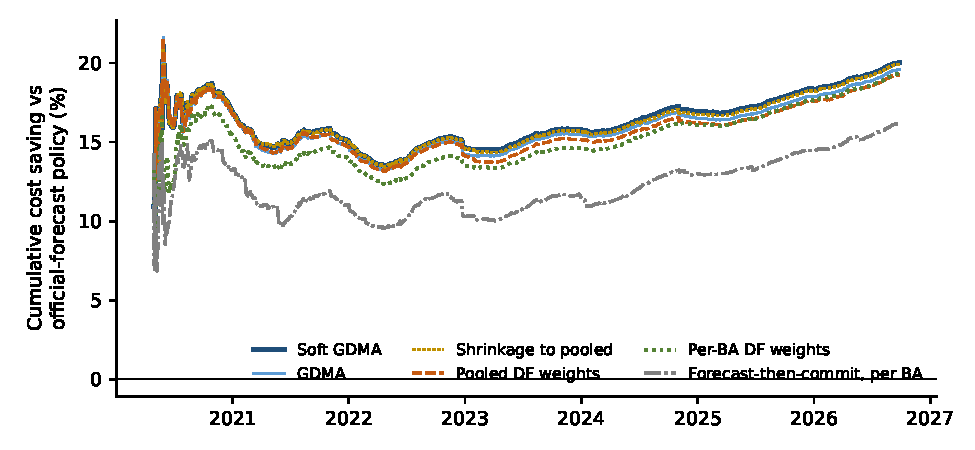
\includegraphics[width=\textwidth]{figures/cumulative.pdf}
\caption{Cumulative system-wide cost saving relative to the official-forecast policy ($W=28$).}\label{fig:cum}
\end{figure}

\subsection{Segments}

\begin{figure}[t]
\centering
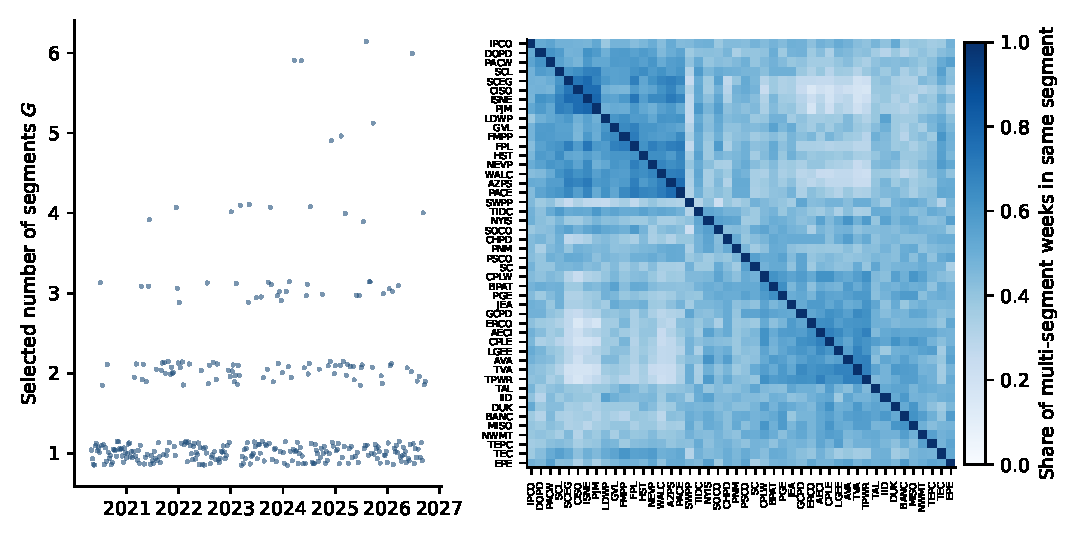
\includegraphics[width=\textwidth]{figures/segments.pdf}
\caption{Left: number of segments selected by GDMA in each weekly re-estimation ($W=28$). Right: among the weeks with $G\ge2$, share of weeks in which two BAs belong to the same segment, ordered by average-linkage clustering.}\label{fig:segments}
\end{figure}

GDMA uses one segment in about two thirds of the weeks and two or more in the rest; multi-segment weeks occur in every year from 2021 onwards (Figure~\ref{fig:segments}, left).
The co-membership matrix (right) reveals two stable segments.
The first contains 17 BAs, among them PJM, CAISO, ISO New England, Florida Power \& Light, Arizona Public Service, Nevada Power and both PacifiCorp areas; their combinations rely almost entirely on the learned models (weights of 0.38 on the hourly regression and 0.47 on LightGBM) and put only 0.12 directly on the official forecast.
The second contains 28 BAs, including MISO, ERCOT, the Southern Company, NYISO, TVA, Bonneville and Duke Energy, and puts 0.39 directly on the official forecast.
Southwest Power Pool often forms a segment of its own.
The two main segments have the same average critical ratio (0.874 and 0.873), so the segmentation is not a relabelling of cost asymmetries; nor does it follow geography or market design, since both contain ISOs and vertically integrated utilities from the East and the West.
What separates them is how much the operator's own forecast adds to what can be learned from recent demand---information that a central planner cannot read off the organisational chart of the grid, but that GDMA extracts from the data.

\subsection{Extreme events and robustness}\label{sec:robust}

\begin{table}[t]
\centering
\caption{System cost during extreme events relative to the official-forecast policy ($W=28$): Winter Storm Uri (10--20 February 2021), Winter Storm Elliott (22--27 December 2022) and the heat wave of 15 July--15 August 2023.}\label{tab:events}
\small
\begin{tabular}{@{}lccc@{}}
\toprule
Method & Winter Storm Uri (10--20 Feb 2021) & Winter Storm Elliott (22--27 Dec 2022) & Heat wave (15 Jul--15 Aug 2023) \\
\midrule
Official forecast & 1.000 & \textbf{1.000} & 1.000 \\
Equal weights & 1.133 & 2.534 & 1.366 \\
Best single (per BA) & 0.881 & 1.264 & 0.796 \\
Pooled DF weights & \textbf{0.842} & 1.318 & \textbf{0.778} \\
Per-BA DF weights & 0.848 & 1.184 & 0.790 \\
Shrinkage to pooled & 0.845 & 1.210 & 0.779 \\
Two-step $k$-means & \textbf{0.842} & 1.239 & 0.780 \\
Forecast-then-commit, per BA & 0.973 & 1.584 & 0.796 \\
Forecast-then-commit, grouped & 0.946 & 1.481 & 0.785 \\
\textbf{GDMA} & \textbf{0.842} & 1.318 & 0.782 \\
\bottomrule
\end{tabular}
\end{table}

Table~\ref{tab:events} examines three extreme episodes.
During Winter Storm Uri and the 2023 heat wave, the decision-focused combinations cost 15--22\% less than the official-forecast policy, in line with their average performance.
Winter Storm Elliott is different: the sudden cold snap of December 2022 was forecast much better by the operators, whose forecasts use weather information that none of our candidates sees directly, and every combination is 18--32\% more expensive than the official policy over those six days.
Soft GDMA and shrinkage limit the damage better than pooled weights and plain GDMA (1.21 against 1.32), presumably because unit-level shrinkage lets the BAs whose official forecasts are most informative keep more weight on them.
The episode is a reminder that combination weights learned in calm weeks cannot anticipate an abrupt regime change; Section~\ref{sec:global} adds candidates driven by archived deterministic and ensemble weather forecasts and shows that they close more than half of this gap.

\begin{table}[t]
\centering
\caption{Sensitivity to the cost asymmetry ($W=28$): system cost relative to the official-forecast policy when every BA has the same critical ratio $\tau$, and under the calibrated heterogeneous ratios.}\label{tab:tau}
\small
\begin{tabular}{@{}lccccc@{}}
\toprule
Method & $\tau=0.5$ & $\tau=0.8$ & $\tau=0.9$ & $\tau=0.95$ & Calibrated \\
\midrule
Official forecast & 1.0000 & 1.0000 & 1.0000 & 1.0000 & 1.0000 \\
Equal weights & 1.4033 & 1.4353 & 1.4860 & 1.5265 & 1.5287 \\
Best single (per BA) & 0.8158 & 0.7921 & 0.8081 & 0.8326 & 0.8245 \\
Pooled DF weights & 0.7988 & 0.7775 & 0.7897 & 0.8136 & 0.8075 \\
Per-BA DF weights & 0.8007 & 0.7798 & 0.7914 & 0.8140 & 0.8069 \\
Shrinkage to pooled & 0.7932 & \textbf{0.7714} & 0.7834 & 0.8067 & 0.8009 \\
Two-step $k$-means & 0.7950 & 0.7736 & 0.7857 & 0.8101 & 0.8041 \\
Forecast-then-commit, per BA & 0.8136 & 0.7944 & 0.8144 & 0.8483 & 0.8382 \\
Forecast-then-commit, grouped & 0.8128 & 0.7916 & 0.8066 & 0.8337 & 0.8260 \\
GDMA & 0.7968 & 0.7750 & 0.7868 & 0.8094 & 0.8042 \\
GDMA, minimum hold-out rule & 0.7981 & 0.7762 & 0.7880 & 0.8098 & 0.8032 \\
\textbf{Soft GDMA} & \textbf{0.7931} & 0.7714 & \textbf{0.7832} & \textbf{0.8065} & \textbf{0.7999} \\
\bottomrule
\end{tabular}
\end{table}

Table~\ref{tab:tau} replaces the calibrated critical ratios by a common $\tau$ for every BA, from the symmetric case $\tau=0.5$ to the highly asymmetric $\tau=0.95$.
The level of the savings changes little---soft GDMA saves 19--23\% relative to the official-forecast policy---and so does the ranking: soft GDMA is the cheapest method for $\tau\in\{0.5,0.9,0.95\}$ and under the calibrated ratios, and ties with shrinkage for $\tau=0.8$.
The advantage of decision-focused over forecast-then-commit combination grows with the asymmetry, from 2.5\% at $\tau=0.5$ to 3.4\% at $\tau=0.95$ relative to the better forecast-then-commit method, as expected: the more asymmetric the cost, the more the best combination for the decision departs from the most accurate one.

\section{Managerial implications and conclusion}\label{sec:conclusion}

\paragraph{Implications for system planners.}
Three lessons emerge for organisations that coordinate many operating units---grid coordinators and regulators, but also national health systems allocating capacity across regions or humanitarian agencies pre-positioning supplies across countries.
First, the object to be learned is the \emph{decision rule}, not the forecast: the cost-minimising combination of forecasting systems depends on the cost asymmetry each unit faces, so a combination tuned for accuracy leaves money on the table.
Second, planners need not choose between a single national rule and a bespoke rule for every unit.
A handful of data-driven segments captures the heterogeneity that matters, is estimated with far less noise than unit-specific rules, and produces a segmentation that can be discussed with operators and regulators---who is grouped with whom, and why.
Third, because GDMA only re-weights rules that operators already produce, it can be adopted without replacing existing forecasting systems, and each unit's commitment remains a convex combination of commitments it already understands.

\paragraph{Limitations and extensions.}
Our cost calibration is stylised: shortfall costs are tied to a transparent proxy of import flexibility rather than to market prices, and the single-period newsvendor abstracts from ramping, network constraints and multi-day commitments.
The timing assumption that the previous day's demand is fully observed before commitment is generous to persistence-type candidates, although all combination methods share the same information.
The theory treats the number of segments as given and relies on a high-level concentration condition; a formal analysis of the hold-out choice of $G$, and of strong cross-sectional dependence through common weather shocks, is left for future work.
Natural extensions include segment-specific weights that vary smoothly with observable states, coupling constraints across units (for example shared reserve pools), and distributionally robust versions of~\eqref{eq:gdma} for periods of rapid structural change.

\paragraph{Conclusion.}
Grouped decision-focused model averaging combines three ideas that have so far developed separately---optimal model averaging, decision-focused learning and latent group structures---into one estimator with finite-sample and asymptotic guarantees.
It gives system planners a principled way to combine the many forecasts they already have into commitment rules that are cheaper, statistically stable and interpretable.


\bibliographystyle{apalike}
\bibliography{refs}

\appendix
\section{Proofs}\label{app:proofs}

Throughout, $\|\cdot\|_1$ is the $\ell_1$ norm and constants $c,C$ may change from line to line.

\paragraph{Covering the simplex.}
For $\epsilon\in(0,1]$ there is a set $\mathcal N_\epsilon\subset\Delta_M$ with $|\mathcal N_\epsilon|\le(3/\epsilon)^M$ such that every $\bm w\in\Delta_M$ has a point $\bm w'\in\mathcal N_\epsilon$ with $\|\bm w-\bm w'\|_1\le\epsilon$ (volumetric argument for the $\ell_1$ ball, e.g.\ \citealp[Ch.~4]{Vershynin2018}).
Hence $\mathcal N_\epsilon^G$ is an $\epsilon$-net of $\Delta_M^G$ in the norm $\max_g\|\bm w_g-\bm w'_g\|_1$, of cardinality at most $(3/\epsilon)^{GM}$.

\paragraph{Lipschitz property.}
For all $(\bm\gamma,\bm W)$ and $(\bm\gamma,\bm W')$ with $\max_g\|\bm w_g-\bm w_g'\|_1\le\epsilon$, Assumption~\ref{as:bounded} gives
$|\widehat R(\bm\gamma,\bm W)-\widehat R(\bm\gamma,\bm W')|\le\bar aB\epsilon$ and $|R(\bm\gamma,\bm W)-R(\bm\gamma,\bm W')|\le\bar aB\epsilon$.

\subsection*{Proof of Theorem~\ref{thm:oracle}}

Fix $\epsilon=1/(NT_e)$.
The set $\mathcal F=\{1,\dots,G\}^N\times\mathcal N_\epsilon^G$ has cardinality at most $G^N(3NT_e)^{GM}$.
By Assumption~\ref{as:concentration} and the union bound,
\[
\Pr\Big(\max_{(\bm\gamma,\bm W)\in\mathcal F}|\widehat R(\bm\gamma,\bm W)-R(\bm\gamma,\bm W)|>x\Big)\le 2G^N(3NT_e)^{GM}\exp(-cNT_ex^2/L^2).
\]
Setting the right-hand side equal to $\delta$ gives, with probability at least $1-\delta$,
$\max_{\mathcal F}|\widehat R-R|\le x_\delta:=L\{(GM\log(3NT_e)+N\log G+\log(2/\delta))/(cNT_e)\}^{1/2}$.
For an arbitrary $(\bm\gamma,\bm W)\in\mathcal P_G$ let $\bm W'$ be its nearest net point; by the Lipschitz property,
\[
\sup_{\mathcal P_G}|\widehat R-R|\le x_\delta+2\bar aB\epsilon .
\]
Let $(\bm\gamma^*,\bm W^*)$ satisfy $R(\bm\gamma^*,\bm W^*)\le R^*_G+\eta$ for arbitrary $\eta>0$.
Since $(\widehat{\bm\gamma},\widehat{\bm W})$ minimises $\widehat R$,
\[
R(\widehat{\bm\gamma},\widehat{\bm W})\le\widehat R(\widehat{\bm\gamma},\widehat{\bm W})+x_\delta+2\bar aB\epsilon
\le\widehat R(\bm\gamma^*,\bm W^*)+x_\delta+2\bar aB\epsilon\le R^*_G+\eta+2x_\delta+4\bar aB\epsilon .
\]
Letting $\eta\downarrow0$ and substituting $\epsilon=1/(NT_e)$ gives~\eqref{eq:oracle}. \qed

\subsection*{Proof of Corollary~\ref{cor:ao}}

Theorem~\ref{thm:oracle} with $\delta=\delta_{N,T}\to0$ slowly (for instance $\log(1/\delta)=\log(NT_e)$) shows $R(\widehat{\bm\gamma},\widehat{\bm W})-R^*_G=O_p(r_{N,T})$ with
$r_{N,T}=\{GM\log(NT_e)/(NT_e)+\log G/T_e+\log(NT_e)/(NT_e)\}^{1/2}\to0$.
Dividing by $R^*_G\ge\kappa$ yields $R(\widehat{\bm\gamma},\widehat{\bm W})/R^*_G-1=O_p(r_{N,T}/\kappa)\to_p0$.
Because $R(\widehat{\bm\gamma},\widehat{\bm W})\ge R^*_N$ always and $R^*_G\ge R^*_N$, the second claim follows once we show $R^*_G=R^*_N$ under the stated structure.
Let $\bm w^0_g$ be a common minimiser of $R_i$ for all $i$ with $\gamma^0_i=g$ (padding with arbitrary vectors if $G_0<G$); then
$R(\bm\gamma^0,\bm W^0)=N^{-1}\sum_i\min_{\bm w}R_i(\bm w)=R^*_N$, so $R^*_G\le R^*_N$, and the reverse inequality holds because $\mathcal P_G$ is a subset of the unit-specific class. \qed

\subsection*{Proof of Theorem~\ref{thm:recovery}}

\emph{Step 1 (average consistency).}
Under Assumption~\ref{as:groups}(a), $R^*_G=R(\bm\gamma^0,\bm W^0)=R^*_N$ and
\[
\frac\lambda N\sum_{i=1}^N\big\|\widehat{\bm w}_{\widehat\gamma_i}-\bm w^0_{\gamma^0_i}\big\|_2^2\le R(\widehat{\bm\gamma},\widehat{\bm W})-R^*_G=o_p(1)
\]
by Theorem~\ref{thm:oracle}, since $\log N/T_e\to0$ implies $\log G/T_e\to0$ and $GM\log(NT_e)/(NT_e)\to0$ for fixed $G$ and $M$.

\emph{Step 2 (consistency of the segment weights).}
Fix $\eta\in(0,d/4)$.
By Step~1 and Markov's inequality, the fraction of units with $\|\widehat{\bm w}_{\widehat\gamma_i}-\bm w^0_{\gamma^0_i}\|_2>\eta$ is $o_p(1)$.
Since every true segment $g$ contains at least $\pi N$ units, with probability approaching one each $g$ contains a unit $i$ with $\|\widehat{\bm w}_{\widehat\gamma_i}-\bm w^0_g\|_2\le\eta$; call $h(g)=\widehat\gamma_i$.
If $h(g)=h(g')$ for $g\ne g'$, the triangle inequality gives $\|\bm w^0_g-\bm w^0_{g'}\|_2\le2\eta<d$, contradicting Assumption~\ref{as:groups}(b).
Thus $h$ is injective, hence a bijection of $\{1,\dots,G\}$, and after relabelling $\max_g\|\widehat{\bm w}_g-\bm w^0_g\|_2\le\eta$ with probability approaching one.
Since $\eta$ is arbitrary, (i) follows.

\emph{Step 3 (memberships).}
On the event $E_\eta=\{\max_g\|\widehat{\bm w}_g-\bm w^0_g\|_2\le\eta\}$, unit $i$ with $\gamma^0_i=g$ can be assigned to $h\ne g$ only if $\widehat R_i(\widehat{\bm w}_h)\le\widehat R_i(\widehat{\bm w}_g)$; every global minimiser assigns each unit to a segment minimising its own empirical cost, since otherwise reassigning the unit would lower~\eqref{eq:gdma}.
By Assumption~\ref{as:groups} and the Lipschitz property (with $\|\cdot\|_1\le\sqrt M\|\cdot\|_2$),
\[
R_i(\widehat{\bm w}_h)-R_i(\widehat{\bm w}_g)\ge\lambda(d-\eta)^2-\bar aB\sqrt M\eta\ge\lambda d^2/4=:\Delta
\]
for $\eta$ small enough.
Hence misclassification of unit $i$ on $E_\eta$ requires $\sup_{\bm w\in\Delta_M}|\widehat R_i(\bm w)-R_i(\bm w)|\ge\Delta/2$.
Covering $\Delta_M$ by $\mathcal N_\epsilon$ with $\epsilon=\Delta/(8\bar aB)$ and applying the unit-level part of Assumption~\ref{as:concentration},
\[
\Pr\Big(\sup_{\bm w}|\widehat R_i(\bm w)-R_i(\bm w)|\ge\Delta/2\Big)\le2\Big(\frac{24\bar aB}{\Delta}\Big)^M\exp\!\Big(-\frac{cT_e\Delta^2}{16L^2}\Big)=:C_M e^{-c'T_e}.
\]
Because the supremum is over all $\bm w$, the bound does not require independence between $\widehat{\bm W}$ and unit $i$'s data.
A union bound over units gives $\Pr(\widehat{\bm\gamma}\ne\bm\gamma^0)\le\Pr(E_\eta^c)+NC_Me^{-c'T_e}$, which tends to zero because $\log N/T_e\to0$. This is (ii).

\emph{Step 4 (oracle equivalence).}
On the event $\{\widehat{\bm\gamma}=\bm\gamma^0\}$, $\widehat{\bm W}$ minimises $\widehat R(\bm\gamma^0,\cdot)$, so $\widehat{\bm W}=\widetilde{\bm W}$ (if the minimiser is not unique, the two estimators select from the same set).
By (ii) this event has probability approaching one. \qed

\section{Out-of-sample risk}\label{app:oos}

The theory concerns the population risk $R$ evaluated at the estimated policy.
In a rolling application the policy estimated on periods $1,\dots,T$ is applied in periods $T+1,\dots,T+k$.
If $\{\bm z_{it}\}$ is $\beta$-mixing with coefficients $\beta(\cdot)$, a coupling argument \citep{Yu1994} shows that the expected cost of the estimated policy in period $T+s$ differs from $\mathbb E\,R(\widehat{\bm\gamma},\widehat{\bm W})$ by at most $L\beta(s)$.
The bounds of Section~\ref{sec:theory} therefore also bound the out-of-sample cost up to a term that vanishes with the gap between estimation and application.

\section{Balancing authorities}\label{app:data}

\begin{table}[h]
\centering
\caption{The 46 balancing authorities, ordered by mean hourly demand over 2019--2026. Flex.: interchange flexibility in 2019 (range between the 5th and 95th percentiles of hourly total interchange, divided by mean demand). $\tau_i$: calibrated critical ratio.}\label{tab:bas}
\scriptsize
\begin{tabular}{@{}llrrr@{}}
\toprule
Code & Balancing authority & Mean MW & Flex. & $\tau_i$ \\
\midrule
PJM & PJM Interconnection, LLC & 92,507 & 0.06 & 0.947 \\
MISO & Midcontinent Independent System Operator, Inc. & 74,189 & 0.07 & 0.943 \\
ERCO & Electric Reliability Council of Texas, Inc. & 49,750 & 0.03 & 0.950 \\
SWPP & Southwest Power Pool & 32,259 & 0.08 & 0.940 \\
SOCO & Southern Company Services, Inc. - Trans & 27,075 & 0.12 & 0.927 \\
CISO & California Independent System Operator & 25,319 & 0.29 & 0.900 \\
TVA & Tennessee Valley Authority & 18,637 & 0.09 & 0.937 \\
NYIS & New York Independent System Operator & 17,306 & 0.18 & 0.910 \\
FPL & Florida Power \& Light Co. & 15,873 & 0.10 & 0.933 \\
ISNE & ISO New England & 13,228 & 0.16 & 0.920 \\
DUK & Duke Energy Carolinas & 12,212 & 0.23 & 0.907 \\
CPLE & Duke Energy Progress East & 7,045 & 0.37 & 0.880 \\
BPAT & Bonneville Power Administration & 6,631 & 0.84 & 0.827 \\
PACE & PacifiCorp East & 5,803 & 0.42 & 0.877 \\
PSCO & Public Service Company of Colorado & 5,312 & 0.11 & 0.930 \\
NEVP & Nevada Power Company & 4,523 & 0.33 & 0.883 \\
LGEE & Louisville Gas and Electric Company and Kentucky Utilities Company & 4,166 & 0.17 & 0.913 \\
AZPS & Arizona Public Service Company & 3,893 & 0.67 & 0.843 \\
SC & South Carolina Public Service Authority & 2,901 & 0.32 & 0.890 \\
LDWP & Los Angeles Department of Water and Power & 2,867 & 0.30 & 0.897 \\
SCEG & Dominion Energy South Carolina, Inc. & 2,814 & 0.15 & 0.923 \\
AECI & Associated Electric Cooperative, Inc. & 2,658 & 0.52 & 0.867 \\
TEC & Tampa Electric Company & 2,530 & 0.26 & 0.903 \\
PGE & Portland General Electric Company & 2,523 & 0.53 & 0.863 \\
PACW & PacifiCorp West & 2,392 & 0.55 & 0.860 \\
FMPP & Florida Municipal Power Pool & 2,135 & 0.17 & 0.917 \\
IPCO & Idaho Power Company & 2,097 & 0.79 & 0.833 \\
BANC & Balancing Authority of Northern California & 1,993 & 0.59 & 0.853 \\
PNM & Public Service Company of New Mexico & 1,645 & 0.64 & 0.847 \\
TEPC & Tucson Electric Power & 1,591 & 0.71 & 0.837 \\
JEA & JEA & 1,532 & 0.32 & 0.893 \\
AVA & Avista Corporation & 1,460 & 0.70 & 0.840 \\
NWMT & NorthWestern Corporation & 1,358 & 1.07 & 0.810 \\
SCL & Seattle City Light & 1,076 & 0.92 & 0.817 \\
WALC & Western Area Power Administration - Desert Southwest Region & 1,045 & 0.95 & 0.813 \\
EPE & El Paso Electric Company & 1,029 & 0.46 & 0.873 \\
GCPD & Public Utility District No. 2 of Grant County, Washington & 696 & 1.58 & 0.807 \\
CPLW & Duke Energy Progress West & 564 & 0.61 & 0.850 \\
TPWR & City of Tacoma, Department of Public Utilities, Light Division & 540 & 0.56 & 0.857 \\
IID & Imperial Irrigation District & 441 & 0.90 & 0.820 \\
TIDC & Turlock Irrigation District & 328 & 0.81 & 0.830 \\
TAL & City of Tallahassee & 322 & 0.32 & 0.887 \\
DOPD & PUD No. 1 of Douglas County & 245 & 2.21 & 0.803 \\
GVL & Gainesville Regional Utilities & 240 & 0.50 & 0.870 \\
CHPD & Public Utility District No. 1 of Chelan County & 218 & 4.71 & 0.800 \\
HST & City of Homestead & 71 & 0.89 & 0.823 \\
\bottomrule
\end{tabular}
\end{table}

\section{Additional results for the global panel}\label{app:global}

\begin{table}[h]
\centering
\caption{Global panel with the main candidate set (eleven candidates including the weather models): system cost relative to the reference forecaster for estimation windows of 14 and 28 days (world).}\label{tab:globalwindows}
\small
\begin{tabular}{@{}lcc@{}}
\toprule
Method & $W=14$ & $W=28$ \\
\midrule
Reference forecaster$^a$ & 1.000 & 1.000 \\
Equal weights & 1.217 & 1.217 \\
Best single (per area) & 0.943 & 0.923 \\
Pooled DF weights & 0.906 & 0.902 \\
Per-area DF weights & 0.918 & 0.895 \\
Shrinkage to pooled & 0.905 & 0.888 \\
Two-step $k$-means & 0.899 & 0.884 \\
Quantile-regression comb. & 1.174 & 1.016 \\
Forecast-then-commit, per area & 1.030 & 0.988 \\
Forecast-then-commit, grouped & 0.990 & 0.966 \\
Neural gate (deep MoE) & -- & 0.956 \\
GDMA & 0.900 & 0.884 \\
\textbf{Soft GDMA} & 0.902 & 0.884 \\
Fair soft GDMA & 0.897 & 0.881 \\
\bottomrule
\end{tabular}
\end{table}

\begin{table}[h]
\centering
\caption{Global panel with the main candidate set and with a common critical ratio $\tau=0.9$ for every grid area ($W=28$): system cost relative to the reference forecaster. The neural gate was not run for this specification.}\label{tab:globaltau}
\small
\begin{tabular}{@{}lcccccc@{}}
\toprule
Method & World & North America & Europe & Oceania & Asia & Africa \\
\midrule
Reference forecaster$^a$ & 1.000 & 1.000 & 1.000 & 1.000 & 1.000 & 1.000 \\
Equal weights & 1.193 & 1.401 & 1.059 & 0.996 & 1.035 & 0.976 \\
Best single (per area) & 0.917 & 0.854 & 0.942 & 1.008 & 1.023 & 0.915 \\
Pooled DF weights & 0.899 & 0.863 & 0.914 & 0.983 & \textbf{0.935} & 0.926 \\
Per-area DF weights & 0.891 & 0.832 & 0.912 & 0.989 & 0.990 & 0.932 \\
Shrinkage to pooled & 0.884 & 0.830 & 0.905 & 0.984 & 0.971 & 0.925 \\
Two-step $k$-means & 0.879 & 0.833 & 0.896 & 0.975 & 0.946 & 0.895 \\
Quantile-regression comb. & 0.987 & 0.945 & 0.987 & 0.983 & 1.179 & 1.064 \\
Forecast-then-commit, per area & 0.958 & 0.934 & 0.932 & 0.989 & 1.184 & 0.946 \\
Forecast-then-commit, grouped & 0.938 & 0.932 & 0.898 & 0.981 & 1.145 & 0.926 \\
GDMA & 0.878 & 0.827 & 0.899 & \textbf{0.973} & 0.954 & \textbf{0.891} \\
\textbf{Soft GDMA} & 0.880 & 0.824 & 0.901 & 0.976 & 0.972 & 0.908 \\
Fair soft GDMA & \textbf{0.876} & \textbf{0.822} & \textbf{0.896} & 0.976 & 0.969 & 0.908 \\
\bottomrule
\end{tabular}
\end{table}


\end{document}
